\documentclass{article}
\usepackage[utf8]{inputenc}
\usepackage{graphics}
\graphicspath{{images/}}

\title{Reversed Arcs}
\author{Vanessa Almelor, Elizabeth Redding, Mansi Sakarvadia}
\break

\date{October 2018}

\begin{document}

\maketitle

\section{Introduction}

\subsection{The Problem}
\begin{flushleft}

An oriented graph is a simple graph where each edge is replaced by an arc (a directed edge). The result is a simple directed graph in which there are no pairs of reversed arcs, meaning that there is only one directed path between any two adjacent vertices.
\break
\break
The square of an oriented graph consists of the original vertices and arcs, but with a single added arc between every two vertices that have a path between them with a length of two, i.e. for each pair of arcs of the form (u, v), (v, w), add the arc (u, w). We determined that the easiest way to model this was by using adjacency matrix for the original oriented graph, and squaring it.
\break
\break
Proposed Conjecture: For every oriented graph, D, there exists a vertex whose out-degree at least doubles when you square the oriented graph.\break
(Note that a vertex with an out-degree of zero fulfills this conjecture if it remains zero in the square of the original graph \(n*0=0,   n \in \Re\).)

\subsubsection{Assumptions Made}
\begin{enumerate}
\item Due to the condition that the square of an oriented graph must include the original arc set, the square of the oriented graph A is in fact $A*A + A$, which we shall refer to as $A^2$. We are aware that using traditional matrices multiplication, $A*A$, would yield a different result and not be representative of the square of our oriented graph. \break

\item We will be working with only connected graphs. If you calculate the square of disconnected components they won’t affect one another. Unproven conjecture: For a disconnected graph, each connected component will in fact have at least one vertex that doubles out-degree after squaring.  \break
\end{enumerate}
\end{flushleft}

\subsection{Terminology}
\begin{flushleft}
\textbf{Adjacency matrix} - A matrix in which a cell (i,j) denotes the number of edges between $v_i$ and $v_j$ \break 
\break
\textbf{Square matrix} - An adjacency matrix in which a cell (i,k) gives the number of paths of length two between  $v_i$ and $v_j$ \break
\break
\textbf{Directed graph} - Set of vertices where edges have direction \break
\break
\textbf{Oriented graph} - Directed graph with no reversed arcs \break
\break
\textbf{Arc} - A directed edge \break
\break
\textbf{Reversed arcs} - Two arcs that are incident to the same pair of vertices and are directed towards different vertices \break 
\break
\textbf{Out-degree} - Total number of arcs originating from and directed away from vertex V \break
\break
\textbf{Chain/One-direction Chain} - Only one path exists between any two vertices on an oriented graph
\end{flushleft}

\subsection{Major Findings}
During our investigation, we came to three main conclusions that satisfy our conjecture. Our first finding is fundamental for the rest of our findings: no vertex can have an out-degree of zero because that vertex will trivially double due to our condition that $n*0=0,n\in\Re$. Additionally, all one-direction cycle graphs and tree graphs follow our conjecture. Finally, we observed that known families of graphs (star graphs, wheel graphs, friendship graphs, and bipartite graphs) fulfill our conjecture through being an extension of a cycle and tree graph. 

\subsubsection{Case 1: No Out-degrees}
Let G be an oriented graph on V vertices where at least one vertex has out-degree zero; let once such vertex be labeled v*. When G is squared, v* will still have an out-degree of zero because no walks exist to any other vertices when starting at v*. The degree doubles because $n*0=0,n\in\Re$, so this trivially proves our conjecture.

\subsubsection{Case 2: Cycle Graphs}
\begin{flushleft}
Let G be an oriented cycle graph, G, on V vertices, where $V\geq3$, and E edges such that $V = E$, and each vertex has and in-degree and out-degree of 1. Thus, G is a cycle graph in which a single path will contain all vertices V.
WLOG, select 3 of the vertices and label them $v_1$, $v_2$, $v_3$, such that there exists two arcs of form ($v_1$,$v_2$) and ($v_2$, $v_3$).
\begin{center}
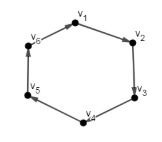
\includegraphics{cycle6.PNG}
\end{center}
\begin{equation}
A  =
\left \{
  \begin{tabular}{cccccc}
  0 & 1 & 0 & 0 & 0 & 0 \\
  0 & 0 & 1 & 0 & 0 & 0 \\
  0 & 0 & 0 & 1 & 0 & 0 \\
  0 & 0 & 0 & 0 & 1 & 0 \\
  0 & 0 & 0 & 0 & 0 & 1 \\
  1 & 0 & 0 & 0 & 0 & 0 \\
  \end{tabular}
\right \}
\end{equation}
Square G.
\begin{center}
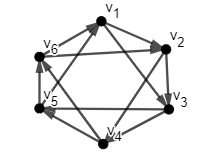
\includegraphics{cycle6square.PNG}
\end{center}
\begin{equation} 
A^2 =
\left \{
  \begin{tabular}{cccccc}
  0 & 1 & 1 & 0 & 0 & 0 \\
  0 & 0 & 1 & 1 & 0 & 0 \\
  0 & 0 & 0 & 1 & 1 & 0 \\
  0 & 0 & 0 & 0 & 1 & 1 \\
  1 & 0 & 0 & 0 & 0 & 1 \\
  1 & 1 & 0 & 0 & 0 & 0 \\
  \end{tabular}
\right \}
\end{equation}
There now exists an arc of form ($v_1$, $v_3$).
Since $v_1$ now has an out degree that connects to both $v_2$ and $v_3$, the out-degree of vertex $v_1$ doubled, which proves our conjecture.\break
\end{flushleft}

\subsubsection{Case 3: Trees and Subtrees}
Let T be an oriented tree graph on V vertices, where $V\geq3$ and E edges, such that T is a connected graph with no cycles and exactly 1 face, F. Trivially, each (sub)tree will have a leaf, which by definition has a degree of 1. Since the (sub)tree is connected, that 1 degree must be an in-degree, leaving the vertex with no out-degree. By \textbf{Case 1}, this gives that every oriented tree graph, T, has at least one vertex that doubles it’s out-degree when squared.

Alternatively, consider a tree graph in which each vertex has an out-degree of at least one. In this case, there must be at least n edges to satisfy the condition, otherwise it is covered by \textbf{Case 1}. However, by definition of a tree graph on n vertices, there must be n-1 edges. Thus, our initial condition is impossible, and there is at least one vertex with an out-degree of 0.

This case trivially applies to star graphs since they are simply a specific type of tree.

\section{Proof}

\begin{flushleft}
Conjecture:  For every oriented graph, G, there exists a vertex whose out-degree at least doubles when you square the oriented graph.\break

If $V=E$, concatenating a tree graph on to a cycle graph will always result in a vertex doubling its out-degree. There are two simple ways to add a tree to a cycle graph:
\begin{itemize}
\item Leaf added to a cycle graph; the vertex at the end of the leaf will have out degree of zero. Trivially proves the proof by \textbf{Case 1}.
\item Arc is added to connect two vertices within the cycle; the new arc creates a smaller cycle with a tree connected, following the same proof as above.

\end{itemize}
\end{flushleft}

\begin{flushleft}

If graph G is a null graph, has $V=1$ or $V=2$ then our conjecture is trivially true by \textbf{Case 1}.

All other possibilities of G will now have $V\geq3$.
\begin{enumerate}
\item Pick a vertex on graph G with an out-degree of at least 1. Let this vertex be $V_1$.
\item Let n be $V_1$’s out-degree. Label each of the outgoing arcs 1 through n.
\item If $V_1$ points to a vertex of no out-degree, \textbf{Case 1} proves our conjecture.
\item If $V_1$ points to a vertex, let this new vertex be called $V_2$.
\item If $V_2$ has no out-degree, case one proves our conjecture.
\item If $V_2$ points to a vertex, let this new vertex be called $V_3$.
\newpage
\item If $V_3$ has no out-degree, \textbf{Case 1} proves our conjecture.
\begin{figure}[ht]
\centering
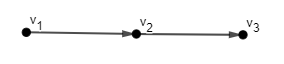
\includegraphics{p3.PNG}
\end{figure}
\item If a one-direction chain exists between $V_3$ and $V_1$, \textbf{Case 2} shows that will at least increase by 1. 
\begin{figure}[ht]
\centering
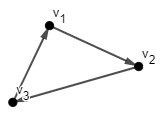
\includegraphics{31.PNG}
\end{figure}
\begin{enumerate}
\item Note: Since we are considering each outgoing arc of $V_1$ separately, we need to show that for each arc being considered at least 1 additional outgoing arc will be added in the squared graph of G. Once we have looped through all of G’s original outgoing arcs with steps 1-7, we will then calculate the outgoing degree sum of $G^2$ which will double since each outgoing arc contributed at least 1 additional outgoing arc in $G^2$.
\end{enumerate}
\item If $V_3$ points to a vertex that is not on a chain with $V_1$, \textbf{Case 3} proves our conjecture.
\begin{figure}[ht]
\centering
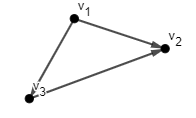
\includegraphics{32.PNG}
\end{figure}
\begin{enumerate}
\item Note: Since we are considering each outgoing arc of $V_1$ separately, we need to show that for each arc being considered at least 1 additional outgoing arc will be added in the squared graph of G. Once we have looped through all of G’s original outgoing arcs with steps 1-7, we will then calculate the outgoing degree sum of $G^2$ which will double since each outgoing arc contributed at least 1 additional outgoing arc in $G^2$.
\end{enumerate}
\item Repeat steps 1 - 7 for all other outgoing arcs of $V_i$ where $0<i\leq n$.

\end{enumerate}
\end{flushleft}

\section{Conclusion}
Throughout this investigation, we have determined that all connected graphs on vertices, V, where $v\geq3$, can be represented by a cycle graph, a tree graph, or a concatenation of the two. In our attempt to prove that all oriented graphs have at least one vertex that doubles its out-degree when we square the original graph, we decided to look at three cases: graphs with at least one vertex with an out-degree of zero, cycle graphs, and tree graphs.

We found that oriented graphs with at least one vertex with an out-degree of zero ($n*0=0,n\in\Re$), providing a basis for other proofs. This allows us to narrow our focus to one-direction cycle graphs which proved trivially true because every vertex gains an arc, thus doubling the out-degree ($1*2=2$). Proving our conjecture for oriented tree graphs took more inspection, but another look at the definition provided the answer we needed. Because trees are defined to be connected graphs with n vertices and n-1 vertices, oriented tree graphs fall under \textbf{Case 1}.

Bringing these case together, we looked at the effect of adding a tree to a cycle. By doing this, the \textbf{Case 3} proof still holds true, and because we know that all graphs are comprised of cycles and trees, our conjecture muse be true for all oriented graphs. Afterwards, we tried to prove this conjecture for other named graphs like bipartite and friendship graphs. We also noticed that adding arcs to connect the vertices in a cycle graph relates to the number of reversed arc pairs in the square of the original oriented graph. Our reasoning for these findings are found in the \textbf{Appendix}.

\section{Appendix}
\subsection{Unproven Conjectures}
\subsubsection{Reversed Arc Conjecture} 
For an oriented cycle graph, G, on v vertices where $v\leq 7$, the number of added arcs is equal to the number of pairs of reversed arcs formed in the squared graph. An example on $C_6$ is shown below where blue indicates the added squared arcs, and red indicates a reversed arc pair:
\begin{figure}[ht]
    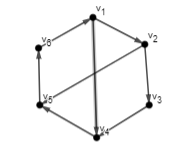
\includegraphics{c6+2.PNG}
    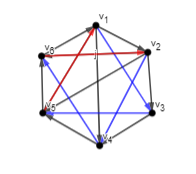
\includegraphics{c6+2sq.PNG}
\end{figure}
This can be explained by noticing that an added arc must "bound" two vertices on the outer edge of the cycle. WLOG, Let $v_1$ refer to a vertex that had an arc added to it. $v_1$ will now have two different paths, one along it's original cycle (to $v_3$), and one following the added arc to $v_4$.  Because the added arc only bounded two vertices, $v_4$ is a walk of length 3 from $v_1$. Continuing the squaring process along the added arc, we arrive at $v_5$, which is a walk of length 2 away from our original vertex $v_1$. We then are left with a reversed arc pair. 
\subsubsection{Bipartite Graphs}
In an oriented bipartite graph, every added edge in the square of the graph will be between two vertices in the same group. In a bipartite graph, every arc must be between two vertices in different groups. Thus, every walk of length 2 from a vertex in group A must lead back to a vertex in group A. 
\begin{figure}[ht]
    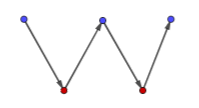
\includegraphics{bipartite.PNG}
    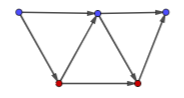
\includegraphics{bipartitesq.PNG}
\end{figure}
\subsubsection{Friendship Graphs}
The square of an oriented friendship graph on n copies of $C_3$, $F_n$ will have 3n pairs of reversed arcs. We know that the square of $C_3$ in which every vertex has at least one out-degree has 3 pairs of reversed arcs. Therefore, every copy of $C_3$ in $F_n$ will yield 3 pairs of reversed arcs, making the total number of reversed arcs in the square of oriented $F_n$, 3n.
\end{document}